%!TEX root = ../Thesis.tex

\chapter{大规模枪支图片数据库的建设}\label{chapter:firearm_dataset}
\section{引言}
在计算机视觉领域的每个研究方向,都存在着一些为大家熟知的数据库,例如,在物体检测与物体分割领域,常用的有 PASCAL VOC 数据库~\cite{Everingham2014ThePV}  以及 Microsoft COCO 数据库~\cite{Lin2014MicrosoftCC};在人脸识别领域,则有 LFW(labeled faces in the wild)~\cite{LFWTech},YTF(YouTube Faces)~\cite{Wolf2011FaceRI} 以及 MegaFace Challenge~\cite{kemelmacher2016megaface}  数据库。一个图片数量丰富,标注准确的数据库,对于推动一个研究领域的发展有着重要的作用。正是由于 PASCAL VOC 数据库和 ImageNet 数据库~\cite{Russakovsky2015ImageNetLS} 的提出,研究者可以在同一数据库用相同的标准比较自己的算法,才推动了研究者对图像分类方法的研究,从而使得图像分类的准确率不断提高,直至超过人类的水平,一个好的数据库对相关研究的推动可见一斑。

图像检索领域,也有一些通用的数据库,最常用的数据库有牛津大学 Visual Geometry Group (VGG)建立的 Oxford building 数据集~\cite{Philbin2007ObjectRW} (简称 Oxford5k),Paris building 数据集~\cite{Philbin2008LostIQ} (简称 Paris6k),法国 INRIA 建立的 Holidays 数据集~\cite{Jgou2008HammingEA} 以及 Nist{\'e}r 和 Stew{\'e}nius 建立的 UKBench 数据集~\cite{Nistr2006ScalableRW} (简称 UKB)。这些数据库的提出时间都较早,建立的时间都在基于深度学习的检索方法兴起之前,因此这些数据库的规模都不是很大,例如 Holiday 数据集只有 1491 张照片,Paris6k 和 Oxford5k 的规模在 5000--6000 张;另外,有的数据库的图片比较简单,例如 UKB 数据集,如图~\ref{fig:ukb_images} 所示,相似图片均是同一物体或场景在不同角度下的照片,因此识别起来相对简单。

在深度学习兴起以后,基于卷积神经网络的图像检索方法也开始流行,众所周知,基于深度学习的方法,在网络的训练过程中往往需要大量的训练图片,否则学习到的模型很容易过拟合,即使我们是在已有的网络的基础上进行微调 (fine-tuning),也需要一定量的图片,才能取得不错的效果。另一方面,在目前的社交网络上,充斥着各种各样的枪支图片,例如许多 Facebook 的用户出于不同的目的在自己的 Facebook 账户上传枪支照片~\cite{Drange2016},这些枪支图片可能会激起暴力,也可能会助长枪支交易的泛滥,因此有必要对枪支图片进行必要的监管与处理。基于这两点考虑,为了方便研究者针对这方面的应用进行研究,我们收集了一个大规模的包含 167 类,总图片数为 14755 的枪支图像数据库,我们将其简称为 Fiream14k。

本章的结构组织如下:\ref{sec:image_collect_clean}节介绍数据库图像的收集与清理过程,\ref{sec:image_label_filtering}节介绍图像的标注,各个标注人员的评分质量评估,以及图像的过滤,\ref{sec:dataset_stats}节介绍枪支数据库的划分(训练集,验证集,测试集),给出各个集合的具体信息,介绍数据库的一些特点,并且给出一些数据库中的示例图片。

\begin{figure}[!t]
	\centering
	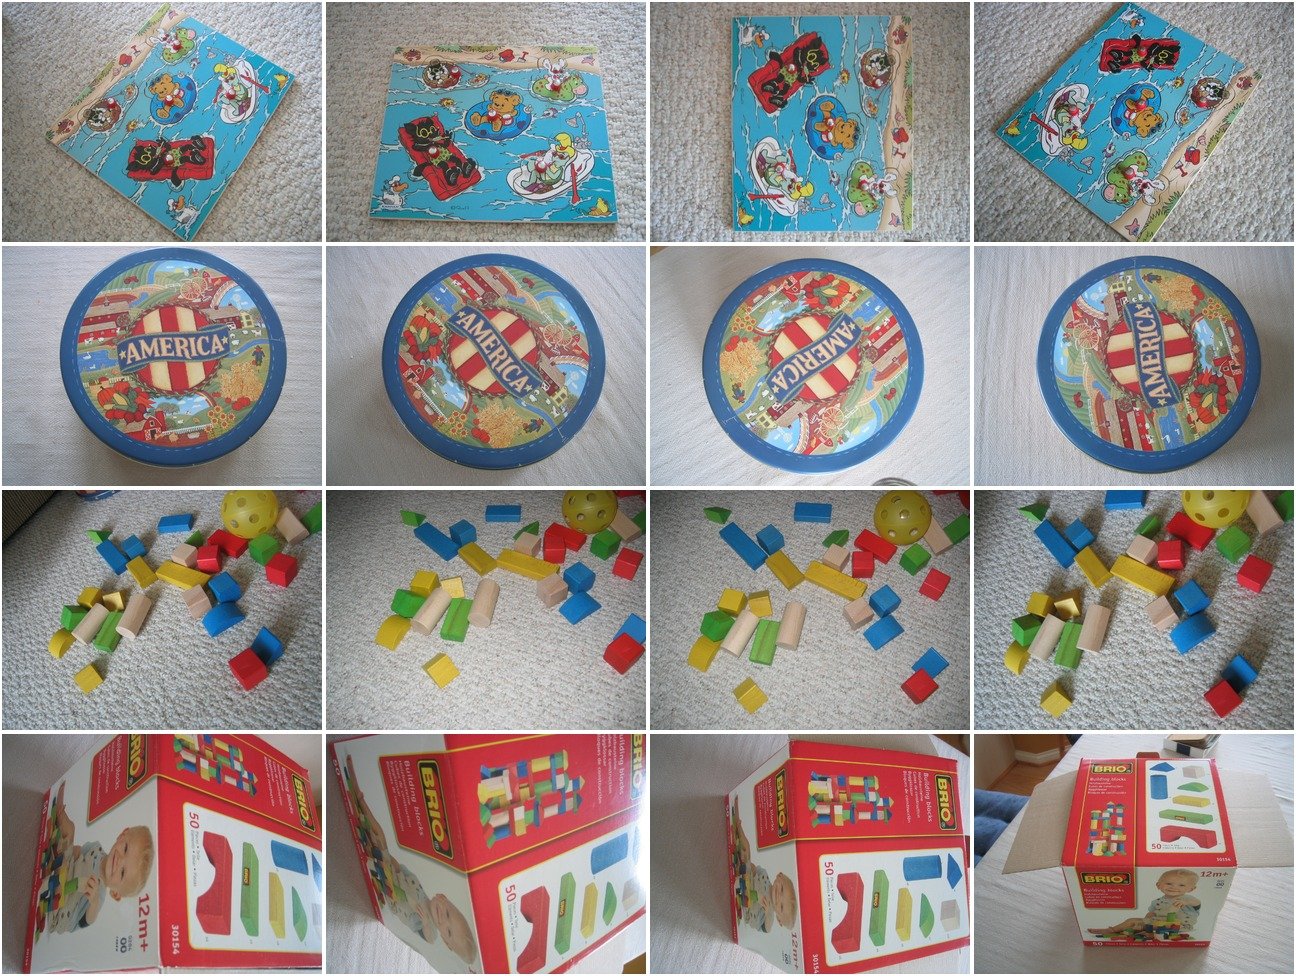
\includegraphics[width=0.9\linewidth]{chapter_firearm_ukb_images.jpg}
	\caption{UKB 数据集中一些示例图片}
	\label{fig:ukb_images}
\end{figure}

\section{图像收集与清理}\label{sec:image_collect_clean}
\subsection{图像的收集}
为了建设我们的枪支数据库,首先我们需要找到一些关键词,我们从一些论坛以及网站搜集了一批枪支名称的关键词。由于一个枪支可能会有很多的不同的型号以及很多仿照的型号,例如,根据维基百科~\footnote{\url{https://en.wikipedia.org/wiki/M16_rifle}},「M16」 这个枪支就有 「M16A2」,「M16A3」,「M16A4」等型号,同时也有一些仿照的枪支,例如 「XM177」。因此有必要处理收集到的关键词列表,去掉重复的关键词。我们认真审查了得到的关键词列表,确保一个枪支和它的不同型号以及仿照枪支不同时出现。经过人工的过滤以后,我们总共得到了 167 个关键词,这些关键词对应着不同的枪支类型,如「来复枪」,「手枪」,「散弹枪」等。

在得到这些枪支名称关键词以后,我们使用谷歌图像搜索引擎~\footnote{\url{https://images.google.com/}},把这些关键词作为查询,提交到搜索引擎。对于每一个关键词,由于对应的枪支类型流行程度不同,因此返回的结果数目也不同,我们使用图片爬虫下载其中 300--500 张图像作为初步的结果。

\subsection{图像的清理}
完成图像的收集以后,我们对图像进行了清理。我们主要去掉了以下几类图片:
\begin{itemize}
\item 损坏的图片(由于下载时候出现的错误)
\item 灰度图片(grayscale images)
\item 最小边小于 128 的小图片
\item 非 JPEG 格式的图片(GIF,TIFF,PNG 等格式)
\end{itemize}

经过图像清理过程,我们总共得到了 62642 张图片,在后续过程中,我们将对这些图片进行人工标注,然后进行评分与过滤,最后得到最终的枪支图片数据库。
\begin{figure}[t]
	\centering
	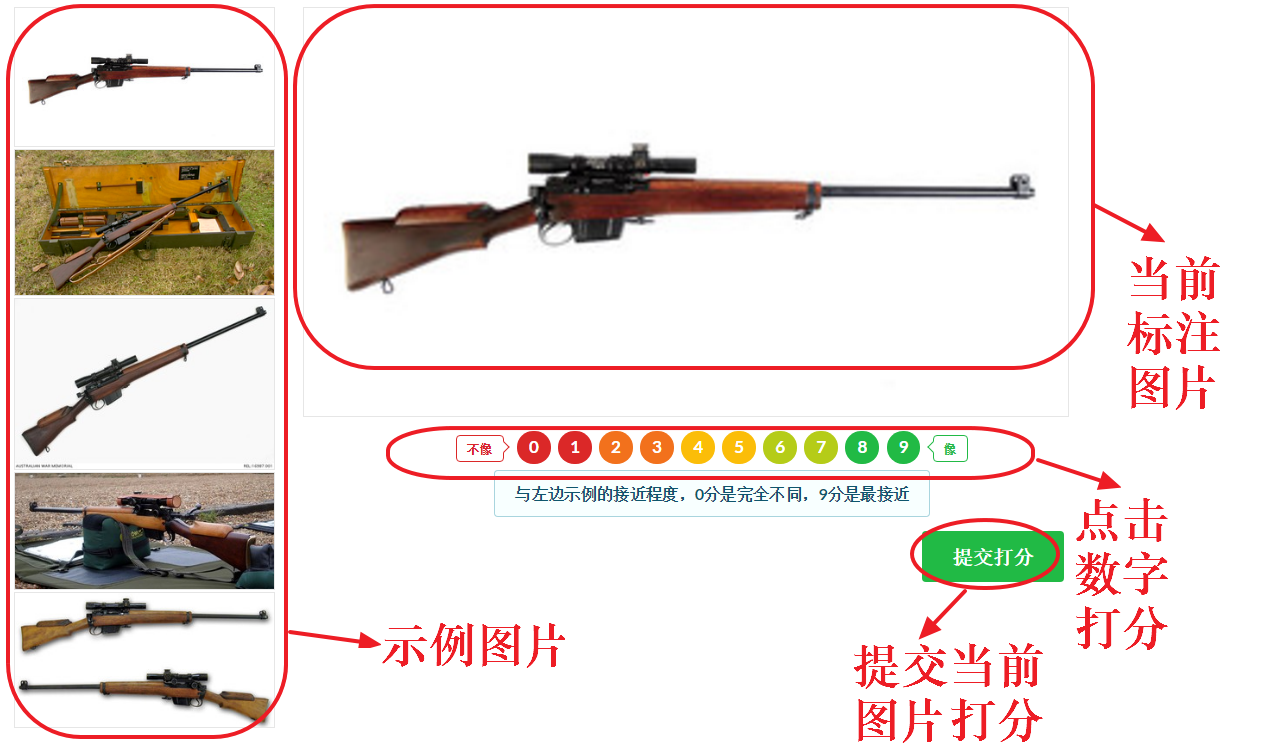
\includegraphics[width=0.9\linewidth]{chapter_firearm_ol_label_system.png}
	\caption{在线图像标注系统的评分界面}
	\label{fig:online_label_system}
\end{figure}

\section{图像标注及质量评估和图像的过滤}\label{sec:image_label_filtering}

\subsection{图像标注}
尽管谷歌的图像搜索引擎根据我们提供的检索词搜索到的图片质量已经相对较高,但是不可避免地,利用检索词搜索到的图片还存在一定的噪声(也就是说,根据某个检索词抓取的图片仍有一部分并不是对应于该检索词),因此我必须要对每一类图片\footnote{我们把通过同一个查询关键词抓取的图片当作一类}进行人工的标注,找出真正属于该类的图片。为了达到这个目的,我们构建了一个简单的在线标注系统,标注人员可以通过网页化的界面 (Web Interface) 对图像进行打分,从而帮助我们找出真正有效的图片。我们的在线标注系统的简单界面如图~\ref{fig:online_label_system}所示。


对于每一类图片,我们实现会人工找出五张真正属于该类的示例图片,然后我们对标注者进行了培训,指导他们标注应该如何进行。在标注过程中,标注者会根据当前要标注的图片(图~\ref{fig:online_label_system}右上部分)与该类的示例图片(图~\ref{fig:online_label_system}左边)的相似程度,对要标注的图片打分,分数范围为 $[0,9]$(0 分代表当前图片与示例图片毫不相关,9 分代表当前图片与示例图片最相似)。我们总共使用了 5 名标注者参与标注工作,每名标注者独立对每一类的所有图片进行打分。因此,在标注人员完成图片标注任务后,对于每一类图片下的每张图片,我们都有 5 个评分。

\subsection{图像标注质量评估}

\begin{figure}[t]
	\centering
	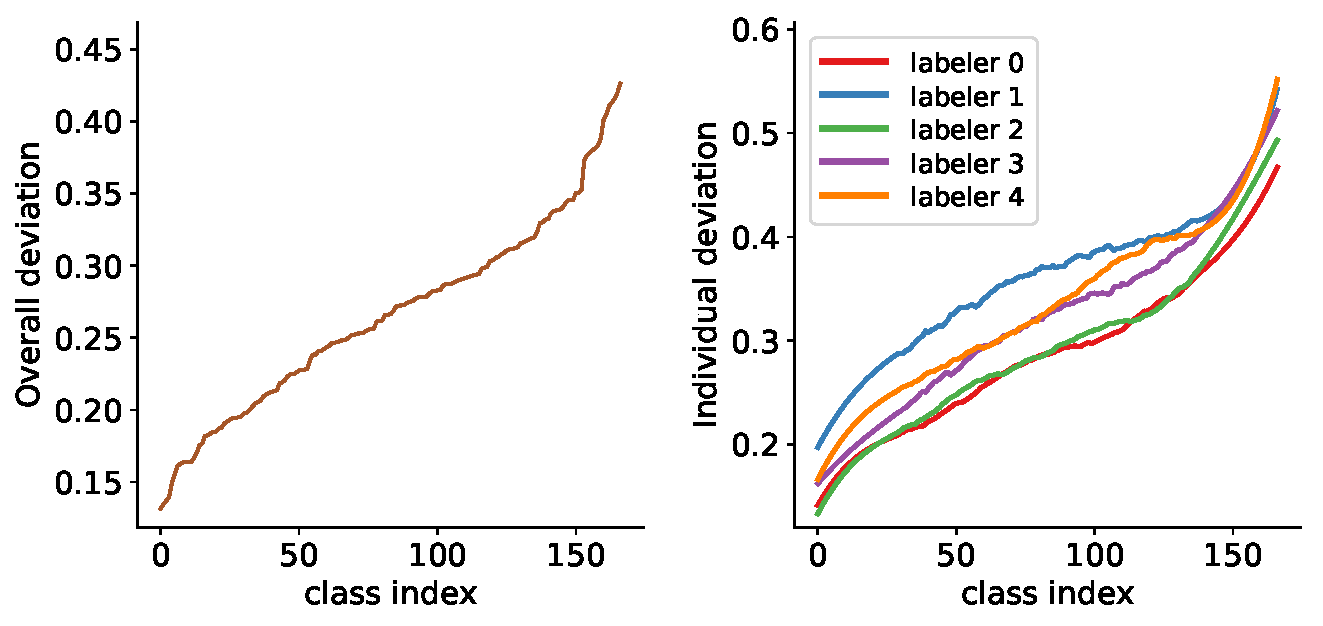
\includegraphics[width=\linewidth]{chapter_firearm_overall_individual_devi.pdf}
	\caption{\textbf{左}:总体的偏差信息;\textbf{右}: 个人的偏差信息}
	\label{fig:deviation_info}
\end{figure}

不可避免地,不同的标注者的标注质量并不是相同的,标注质量的高低取决于很多因素,例如,标注者在标注过程中是否认真以及标注者对于相似的认识也可能有差异。为了给每一类下的每一张图片一个可靠的评分,我们必须科学地对标注者的标注质量进行评估。

首先,对于每一类图像,我们计算出不同打分者的打分之间的相关系数,我们用一个对称矩阵 $C$ 来表示相关性信息。矩阵 $C$ 的大小为 $5\times 5$,每个元素 $C[i,j]$ 代表第 $i$ 个标注者与第 $j$ 个标注者的评分之间的相关性。在理想情况下,两个标注者对某一类下面的图片评分肯定会有所不同 (某个图片的具体评分值可能会有不同),但是他们的打分相关性应该足够高,因此矩阵 $C$ 的每个元素都应该接近 1。如果一个标注者标注的质量不高,那么他/她的评分和其他人的评分之间的相关关系就会比较弱,我们可以据此定义每一类的总的偏差(overall diviation,OD)和个人偏差(individual deviation,ID)。对于某一类图片,总的偏差可以定义为:
\begin{equation}
OD = \frac{15 - \sum_{i=0}^{4}\sum_{j=i}^{4}C[i,j]}{15}\, ,
\end{equation}
对于标注者 $i$,个人偏差可以定义为:
\begin{equation}
	ID[i] = \frac{5 - \sum_{j=0}^{4}C[i, j]}{5}\, .
\end{equation}
在以上两个公式中,$C$ 是对应与某类的相关性矩阵。

在图~\ref{fig:deviation_info}中,我们展示了偏差信息的总体分布情况与个人分布情况:左图展示的总体的偏差分布情况,我们把偏差按照从小到大进行了排序;右图展示的是对应于每个人的偏差分布情况\footnote{为了滤除一些噪声,显示出趋势,我们对曲线进行了一定的平滑处理},和总体偏差采用了相同的类别编号顺序。一个标注者在某类上偏差越大,那么他在该类上的评分就越不可靠。从图~\ref{fig:deviation_info}中可以看出,标注者 1 在整体上有着最大的偏差(这意味着比较差的标注质量),标注者 3 和 4 相对来说,偏差较小,因此他们的标注质量较好,标注者 0 和 2 的总体偏差最小,因此他们的标注质量是最好的。

然后,我们统计了每个标注者在多少个类别上具有最大的个人偏差,这个指标可以用来衡量每个人的评分质量。在表~\ref{table:largest_devi_num}中,我们列出了统计数据。从中可以看出,在所有的 167 类中,标注者 1 在其中 93 类有最大的偏差值,这表明标注者 1 总体的标注质量很差;标注 3 和 4 在其中 33 类上有最大偏差值,这表明他们的标注质量中等,对于标注者 0 和 2,他们分别只在 167 类中的 9 类有最大的偏差值,这表明他们的标注质量是极其优秀的。
\begin{table}[!t]
	\centering
	\caption{每个标注者有最大的个人偏差的类别数目}
	\begin{tabular}{@{}llllll@{}}
		\toprule
		标注者编号	    &  0		& 1 & 2 & 3 & 4  \\
		\midrule
		数目 &  4 & 93 & 4 & 33 & 33 \\
		\bottomrule
	\end{tabular}
	\label{table:largest_devi_num}
\end{table}

\begin{figure}[t]
	\centering
	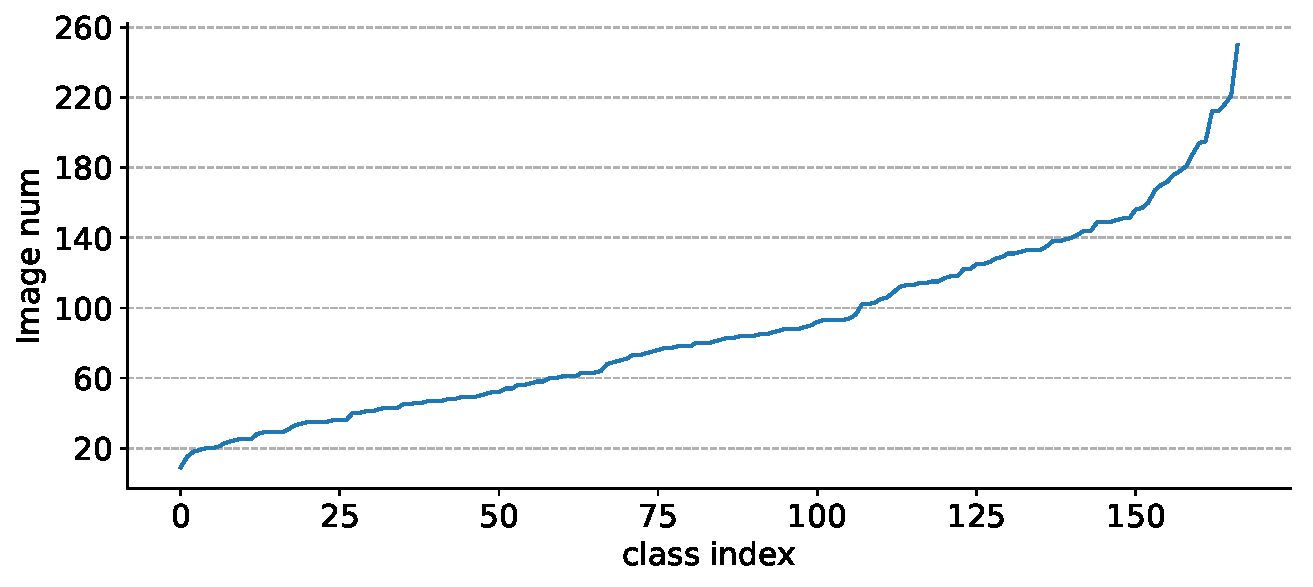
\includegraphics[width=\linewidth]{chapter_firearm_dataset_cls_img_num.pdf}
	\caption{枪支图像数据库各个类别图片数量}
	\label{fig:dataset_cls_img_num}
\end{figure}

\subsection{图像过滤}
为了选出每一类的真正有效的图片,我们需要选出和给出的示例图片相似性得分高的图片。对于每一类别下的每张图片,我们使用五个标注者打分的加权平均分作为每张的图片的相似性得分。由于标注者 1 的评分质量太低,我们把标注者 1 的权重设为了 0,对于其他标注者,权重反比于他/她在多少类上有最大的个人偏差,这些权重之和为 1,我们最终使用的权重为

 \[w = [0.445, 0, 0.445, 0.055, 0.055]\]

对于每类下的每张图片,其最终的相似性得分 $s$ 为

\begin{equation}
s = \sum_{i=0}^{4}w_{i}s_{i}\, ,
\end{equation}

其中 $s_i$ 表示第 $i$ 个标注者对图片的评分。然后我们选择相似性得分在 6 分以上(含 6 分)的图片作为每类的有效图片,这些图片构成了我们的枪支数据库。

\section{数据库的划分与相关统计信息}\label{sec:dataset_stats}


最终,我们得到的枪支数据库含有 14755 张图片,这些图片来自 167 类不同类型的枪支,我们将该数据库命名为 Firearm14k。该数据库有两个值得注意的特点:
\begin{itemize}
\item  该数据库具有高度不平衡 (imbalanced)的特点(图~\ref{fig:dataset_cls_img_num}展示了数据库中各类的图片数目,按照图片数目从小到大排序),有的类别的图像包含的图片数目超过 200,还有一些类别图片数量大约只有 20 左右。
\item 该数据库中的图片是从真实世界中得到,因此图片中的枪支在尺度,拍照的视角,姿态,光照等因素的变化,背景也十分复杂,因此识别的难度很大。
\end{itemize}
在图~\ref{fig:dataset_sample_images}中,我们展示了一些随机选取自枪支数据库的示例图片,从图中可以看出,这些枪支图片中枪支的尺寸,拍摄的视角等变化千差万别,这给枪支图片的识别带来了很大的困难,也是我们试图解决的问题。

\begin{figure}[t]
	\centering
	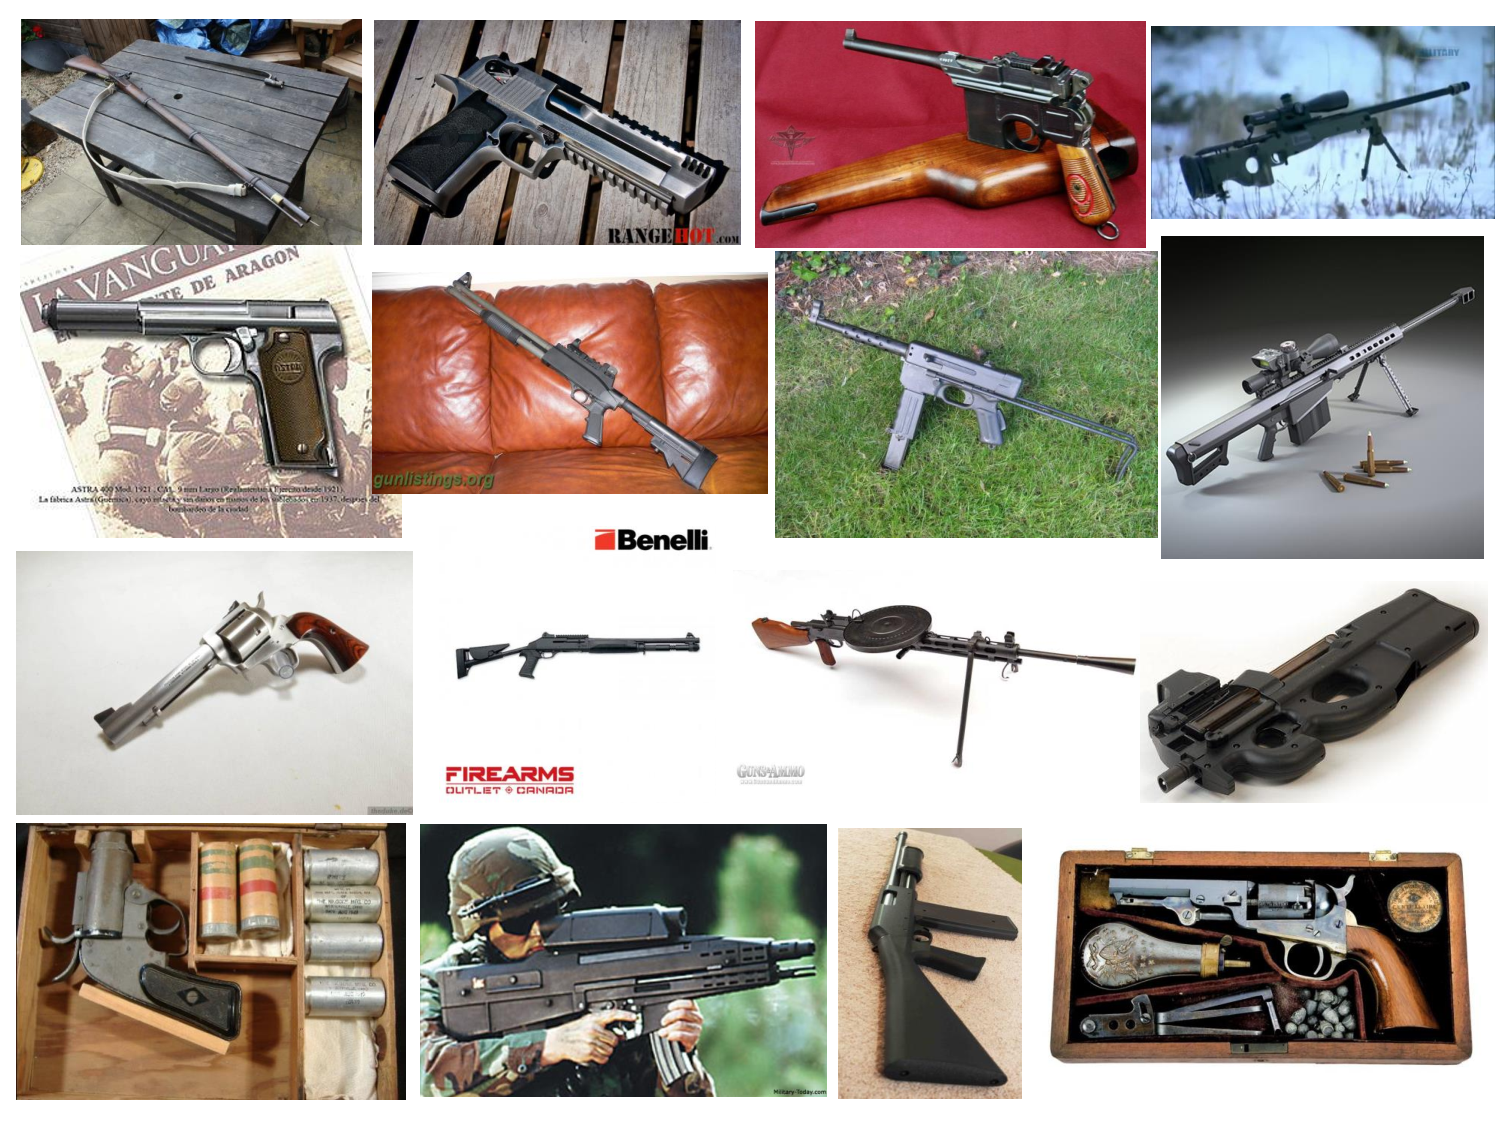
\includegraphics[width=\linewidth]{chapter_firearm_dataset_images.pdf}
	\caption{来自 Firearm14k 数据库的一些示例图片}
	\label{fig:dataset_sample_images}
\end{figure}

我们把数据库划分为训练集,验证集以及测试集,每个集合分别占总的图片量的大约 65\%,10\% 和 25\%,为了模拟真实的检索场景,三个集合的图片类别互不交叉 (具体做法是把 167 类图片随机划分为 3 个互不相交的集合,使得三个集合的图片数目占总图片量的比例接近预定的比例)。我们在表~\ref{table:train_val_test_stat}第 2 行与第 3 行列出了三个集合的图片类别数目,图像数目。对于验证集和测试集,我们从每一类图片中随机选择了两张作为查询图片\footnote{验证集的查询图像中,有一张标注有错误,我们从查询图片中去掉了该图片},我们把剩余的所有图片作为分别作为验证集和测试集的搜索图像库,具体的图片数目信息见表~\ref{table:train_val_test_stat}第 4 行和第 5 行。

\begin{table}[!t]
	\centering
	\caption{训练集,验证集以及测试集类别数目,图像总数,查询图片以及图片库图片数目}
	\begin{tabular}{@{}llll@{}}
		\toprule
		          & 训练集 & 验证集 & 测试集 \\
		\midrule
		类别数目 & 107       & 20             & 40       \\
		图片数目 & 9628      & 1478           & 3649     \\
		查询图片数目 & --        & 39             & 80       \\
		图片库 (database)图片数目 & -- & 1438 &  3569 \\
		\bottomrule
	\end{tabular}

	\label{table:train_val_test_stat}
\end{table}

\section{本章小节}
本章主要介绍了我们的枪支图片数据库的构建过程。首先,我们介绍了枪支图片的收集与清理,然后我们介绍了图像的标注过程,以及以相关性系数矩阵为基础,确定标注者的标注质量,进而得到图片的相似度分数,从而筛选出每一类真正有效的图片。最后,我们介绍了数据库的划分,并给出了数据库的详细统计信息。
